\documentclass[11  pt]{article} 
\usepackage[lmargin=1in,rmargin=1.75in,bmargin=1in,tmargin=1in]{geometry}
\usepackage[T1]{fontenc}
\usepackage{amsmath,amssymb,amsthm}
\usepackage{enumitem,array,booktabs,fancyhdr}
\usepackage[hidelinks]{hyperref}


% For hyperlinking everything
\usepackage{hyperref}
\hypersetup{
	colorlinks=true, %set true if you want colored links
	linktoc=all,     %set to all if you want both sections and subsections linked
	linkcolor=blue,  %choose some color if you want links to stand out
}


\usepackage[latin1]{inputenc}
\usepackage{amsmath}
\usepackage{mathrsfs}  
\usepackage{amsfonts}
\usepackage{amssymb}
\usepackage{graphicx}
\usepackage{subfig}
\usepackage{caption}
\usepackage{algorithm}
%\usepackage{algcompatible}
%\usepackage{algorithmicx}
\usepackage{algpseudocode}

\usepackage{titlesec}
\titleformat{\section}{\fontfamily{lmss}\fontsize{14}{15}\bfseries}{\thesection}{1em}{}
\titleformat{\subsection}{\fontfamily{lmss}\fontsize{12}{15}\bfseries}{\thesubsection}{1em}{}




\usepackage{amsthm}

\newtheoremstyle{noit}
{10pt}% <Space above>
{10pt}% <Space below>
{}% <Body font>
{}% <Indent amount>
{\bfseries}% <Theorem head font>
{.}% <Punctuation after theorem head>
{.5em}% <Space after theorem headi>
{}% <Theorem head spec (can be left empty, meaning `normal')>

\newtheoremstyle{example}
{10pt}% <Space above>
{10pt}% <Space below>
{}% <Body font>
{20pt}% <Indent amount>
{\bfseries}% <Theorem head font>
{.}% <Punctuation after theorem head>
{.5em}% <Space after theorem headi>
{}% <Theorem head spec (can be left empty, meaning `normal')>


\newtheoremstyle{indented}{20pt}{20pt}{\addtolength{\leftskip}{2.5em}}{}{\bfseries}{.}{.5em}{}


\newtheorem{theorem}{Theorem}
\numberwithin{theorem}{section}
\newtheorem{lemma}[theorem]{Lemma}
\newtheorem{corollary}[theorem]{Corollary}
\newtheorem{observation}{Observation}
%\numberwithin{observation}{section}
%\numberwithin{definition}{section}
\newtheorem{conjecture}{Conjecture}
\newtheorem{Qu}{Question}
\newcommand{\QU}{\begin{Qu}\normalfont}

\theoremstyle{noit}
\newtheorem{fact}{Fact}
\newtheorem{definition}{Definition}

\theoremstyle{indented}
\newtheorem{example}{Example}

\theoremstyle{indented}
\newtheorem{problem}{Problem}


%\newenvironment{proof}{\noindent{\bf Proof:} \hspace*{1em}}{
%    \hspace*{\fill} $\Box$ }
%\newenvironment{proof_of}[1]{\noindent {\bf Proof of #1:}
%    \hspace*{1em} }{\hspace*{\fill} $\Box$ }
%\newenvironment{proof_claim}{\begin{quotation} \noindent}{
%    \hspace*{\fill} $\diamond$ \end{quotation}}
\newcommand{\vs}[1]{\vspace{#1}}

\newcommand{\lecture}[2]{
 \noindent
\begin{center}
	\framebox{
		\vbox{
			\hbox to 5.78in { {\bf CSCE 411: Design and Analysis of Algorithms (Honors)} \hfill  }
			\vspace{2mm}
			\hbox to 5.78in { {\Large \hfill Lecture #1\hfill} }
			\vspace{2mm}
			\hbox to 5.78in { {\it Date: #2 \hfill Samson Zhou} }
		}
	}
\end{center}
\vspace*{4mm}
}

\newcommand{\week}[2]{
 \noindent
\begin{center}
	\framebox{
		\vbox{
			\hbox to 5.78in { {\bf CSCE 411: Design and Analysis of Algorithms (Honors)} \hfill  }
			\vspace{2mm}
			\hbox to 5.78in { {\Large \hfill Week #1\hfill} }
			\vspace{2mm}
			\hbox to 5.78in { {\it Date: #2 \hfill Nate Veldt, updated by Samson Zhou} }
		}
	}
\end{center}
\vspace*{4mm}
}

\newcommand{\sweek}[2]{
 \noindent
\begin{center}
	\framebox{
		\vbox{
			\hbox to 5.78in { {\bf CSCE 411: Design and Analysis of Algorithms (Honors)} \hfill  }
			\vspace{2mm}
			\hbox to 5.78in { {\Large \hfill Week #1\hfill} }
			\vspace{2mm}
			\hbox to 5.78in { {\it Date: #2 \hfill Samson Zhou} }
		}
	}
\end{center}
\vspace*{4mm}
}

\newcommand{\hw}[2]{
	\noindent
	\begin{center}
		\framebox{
			\vbox{
				\hbox to 5.78in { {\bf CSCE 411: Design and Analysis of Algorithms} \hfill  }
				\vspace{2mm}
				\hbox to 5.78in { {\Large \hfill Homework #1\hfill} }
				\vspace{2mm}
				\hbox to 5.78in { {\it Due date: #2 \hfil} }
			}
		}
	\end{center}
	\vspace*{4mm}
}



\newcommand{\under}[1]{\underline{\hspace{#1}}}
\setlength{\parindent}{0em}

%\usepackage[tagged]{accessibility}

% Graph terms
\newcommand{\vol}{\textbf{vol}}
\newcommand{\cut}{\textbf{cut}}


% Matrices
\newcommand{\mA}{\textbf{A}}
\newcommand{\mB}{\textbf{B}}

% vectors
\newcommand{\ve}{\textbf{e}}
\newcommand{\vx}{\textbf{x}}


% Other
\newcommand{\calN}{\mathcal{N}}

\usepackage{mathtools}
\DeclarePairedDelimiter\ceil{\lceil}{\rceil}
\DeclarePairedDelimiter\floor{\lfloor}{\rfloor}


\newcommand*{\aitem}{ \item[{
\includegraphics[width=0.8cm,height=0.5cm]{figures/A}} ]  }
\newcommand*{\bitem}{ \item[{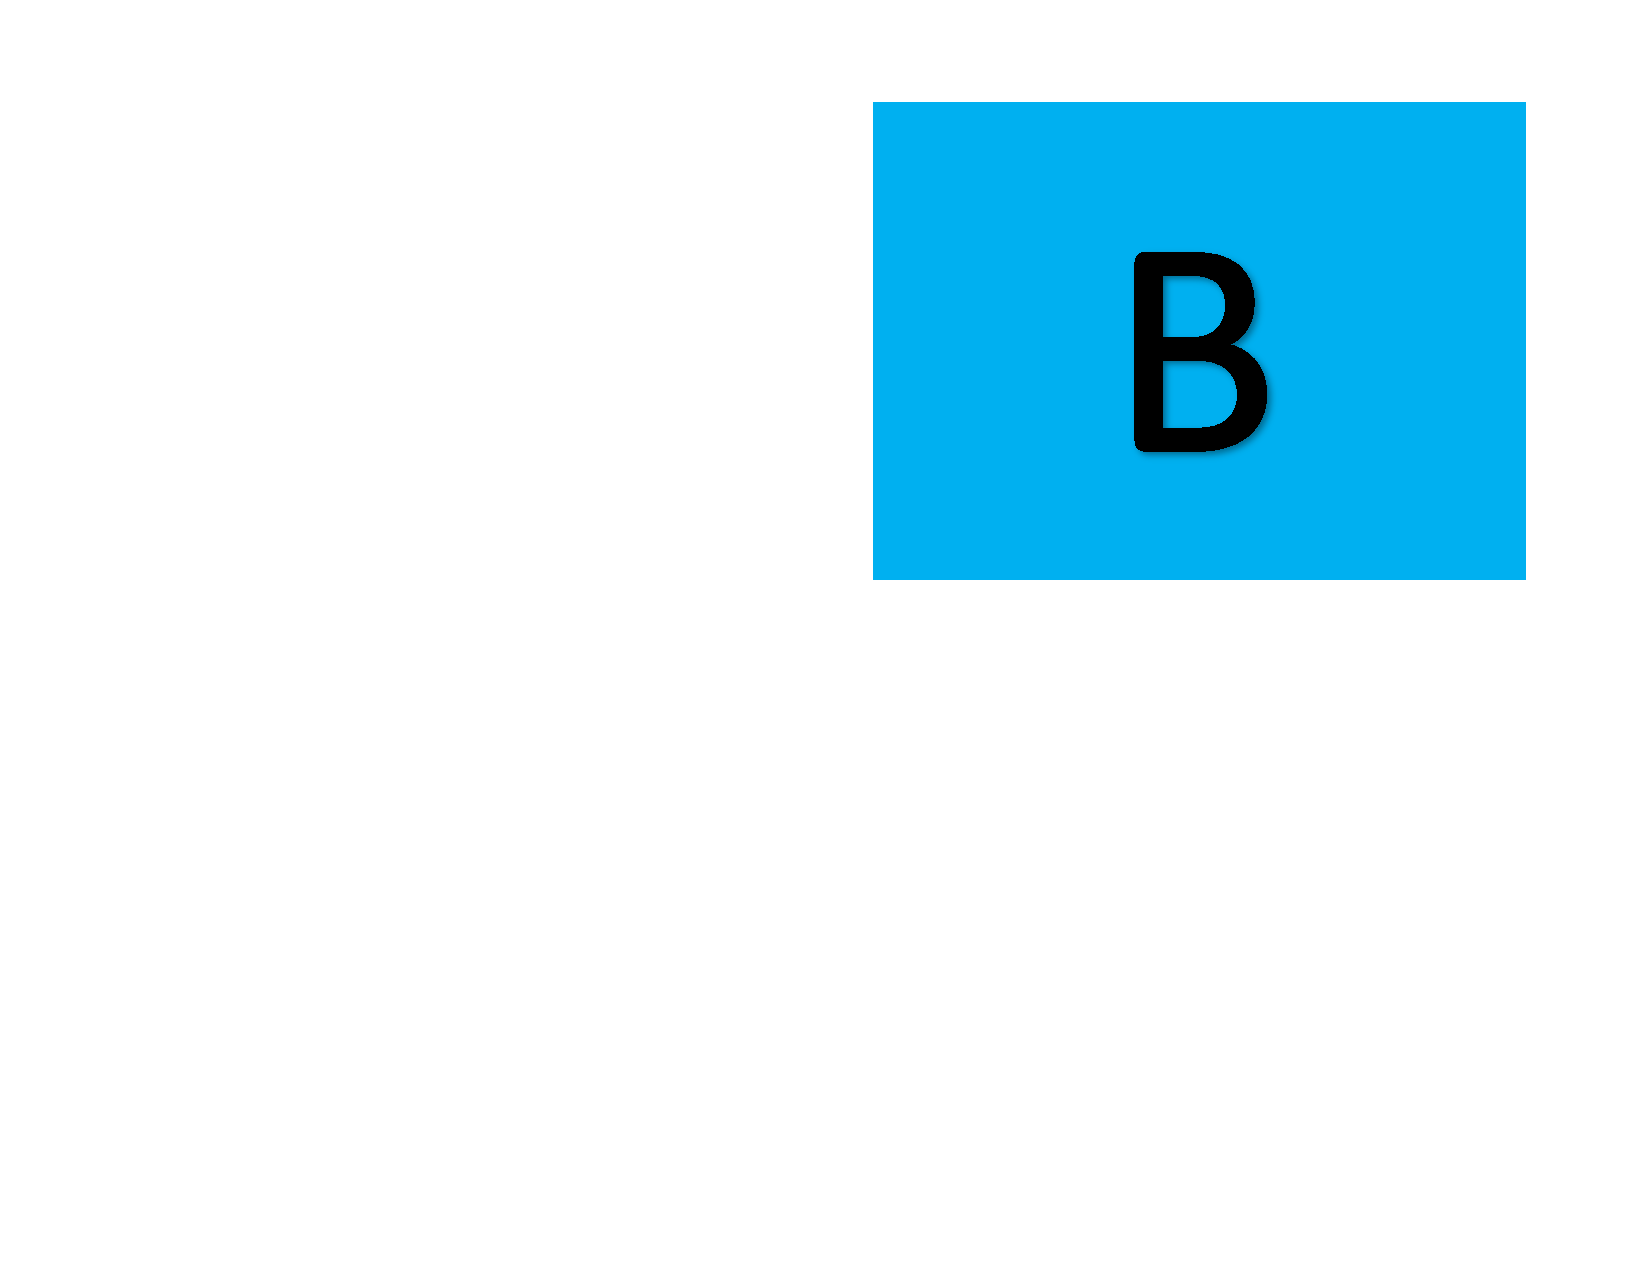
\includegraphics[width=0.8cm,height=0.5cm]{figures/B}} ]  }
\newcommand*{\citem}{ \item[{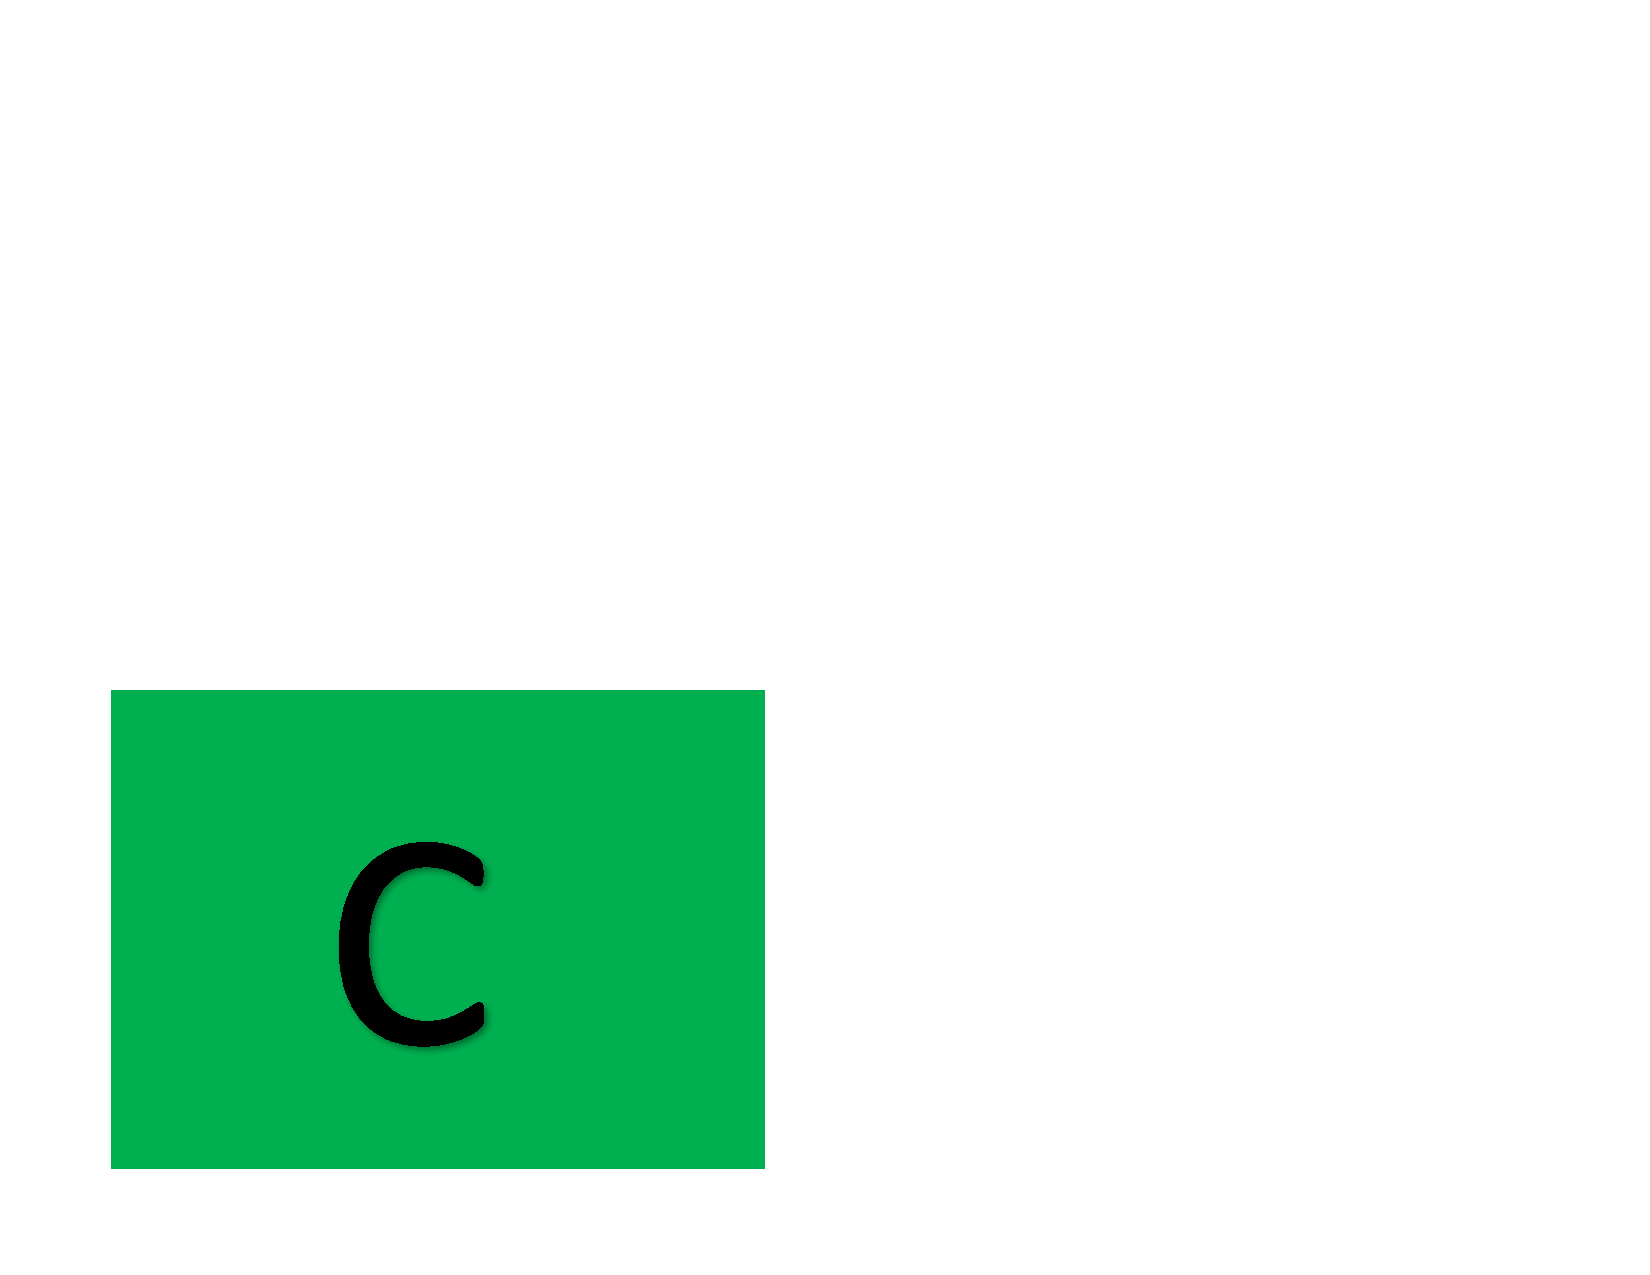
\includegraphics[width=0.8cm,height=0.5cm]{figures/C}} ]  }
\newcommand*{\ditem}{ \item[{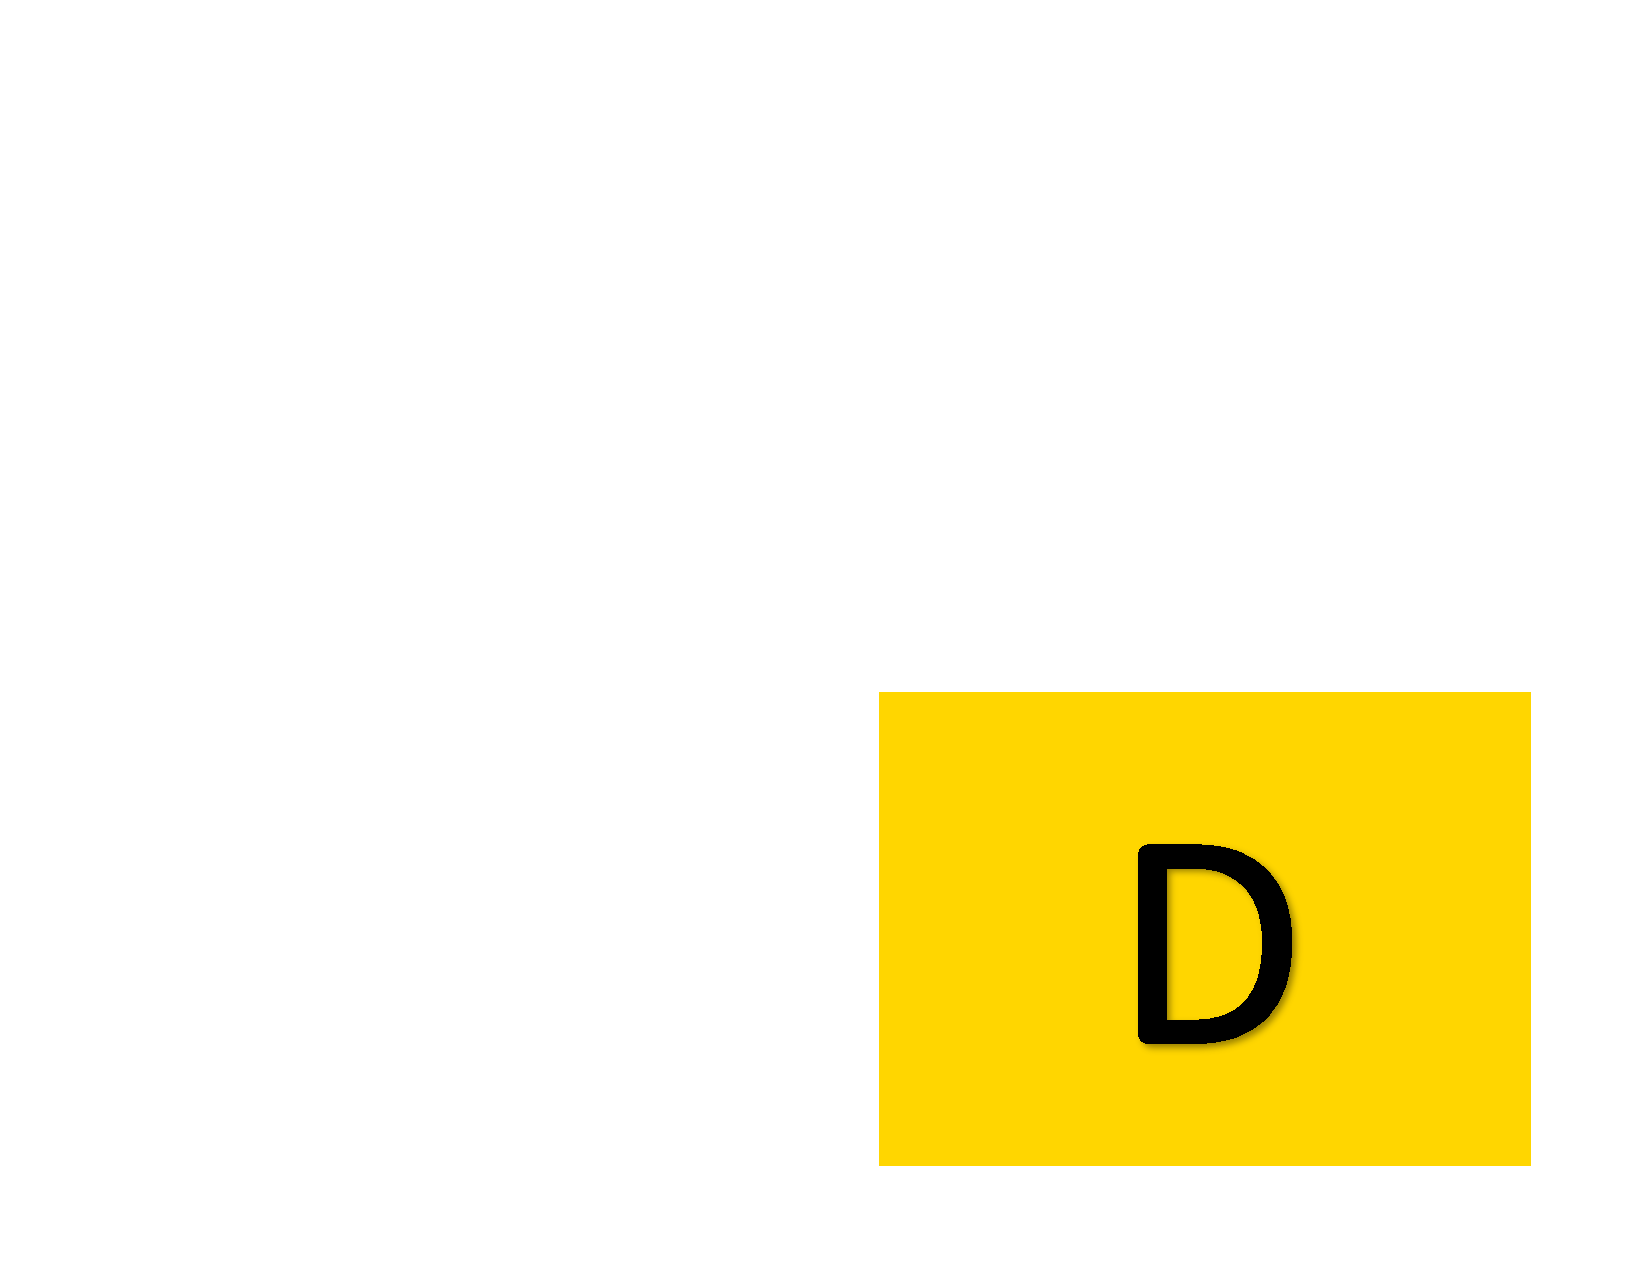
\includegraphics[width=0.8cm,height=0.5cm]{figures/D}} ]  }
\newcommand*{\eitem}{ \item[{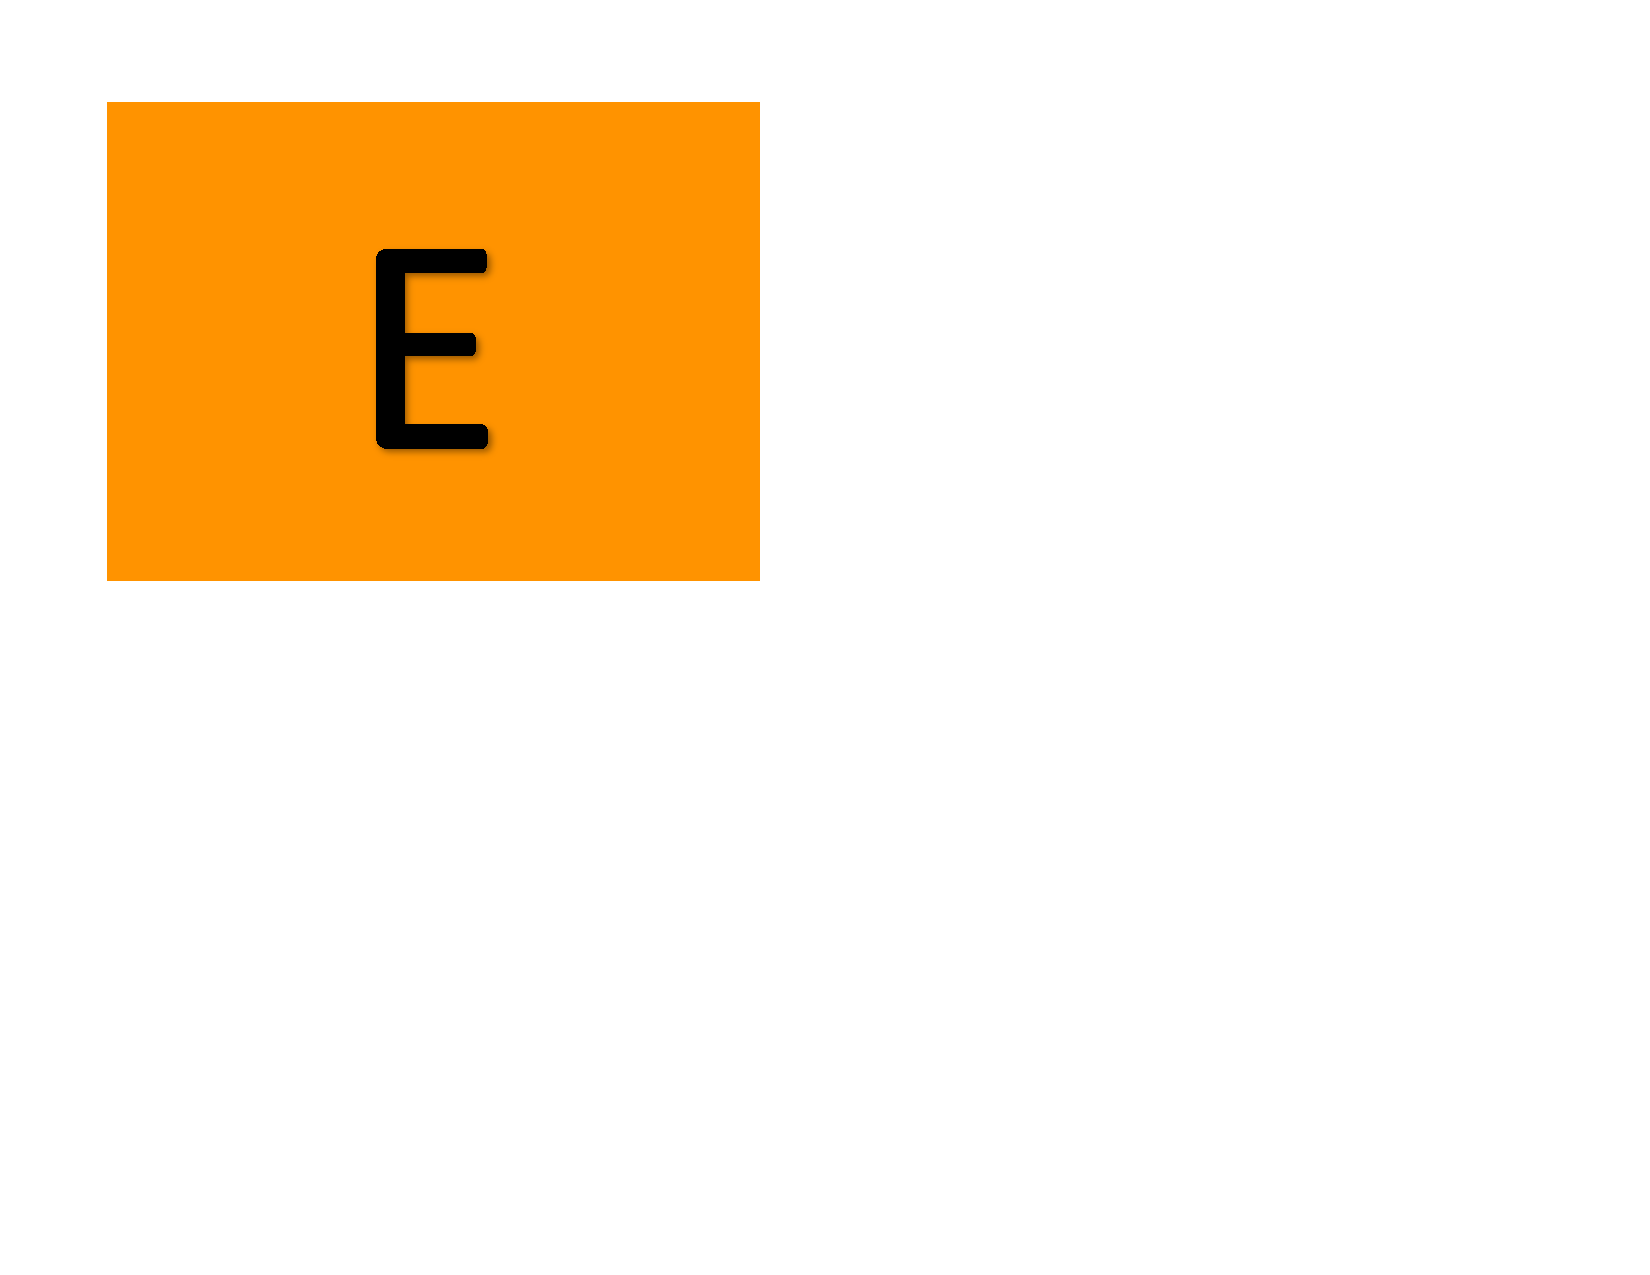
\includegraphics[width=0.8cm,height=0.5cm]{figures/E}} ]  }
\newcommand*{\fitem}{ \item[{
\includegraphics[width=0.8cm,height=0.5cm]{figures/F}} ]  }


\newcommand{\hide}[1]{\underline{\phantom{#1 #1}}}

\usepackage{setspace}

\onehalfspacing

\begin{document}
\sweek{7: All-Pairs Shortest Paths}{October 6, 2026}

\paragraph{Today's questions}
How do we find a shortest path between \emph{every} pair of vertices?
How do we know whether an algorithm can be improved?
What does this have to do with cutting a steel rod?

\section{The All-Pairs Shortest Paths Problem}
Let $G=(V,E,w)$ be a directed, weighted graph with $V=\{1,\ldots,n\}$.
We allow negative edge weights, but assume that there are \textbf{no negative-weight cycles}.
As before, $\delta(i,j)$ is the minimum weight of an $i$-to-$j$ path,
or $\infty$ if no such path exists. The empty path has weight $0$.

\paragraph{Definition}
The \emph{all-pairs shortest paths} (APSP) problem asks us to compute
$\delta(i,j)$ for \hide{every ordered pair $i,j\in V$}.
The output is an $n\times n$ table of distances.

\subsection{Choosing the right subproblems}
An \emph{internal vertex} of a path is any vertex other than its endpoints.
Let
\[
 D^{(k)}[i,j]=\text{minimum weight of an $i$-to-$j$ path whose}
\]
\[
 \text{internal vertices belong to $\{1,\ldots,k\}$.}
\]
The indices $i,j$ may be any vertices, even if they are larger than $k$.
With no internal vertices allowed, the path is empty or uses one edge:
\[
 D^{(0)}[i,j]=
 \begin{cases}
  0 & i=j,\\
  w(i,j) & i\ne j\text{ and }(i,j)\in E,\\
  \infty & \text{otherwise.}
 \end{cases}
\]
If parallel edges occur, use their minimum weight.

\begin{Qu}
When we allow vertex $k$ as an internal vertex, what are the two possibilities
for a shortest path from $i$ to $j$?
\end{Qu}
\vspace{2in}
%\hide{It avoids $k$, or it goes through $k$. In the second case,
%split the path at $k$ into an $i$-to-$k$ part and a $k$-to-$j$ part.}
\[
\boxed{D^{(k)}[i,j]=\hide{\min\bigl\{D^{(k-1)}[i,j],\ D^{(k-1)}[i,k]+D^{(k-1)}[k,j]\bigr\}.}}
\]

\vspace{2in}

\section{The Floyd--Warshall Algorithm}
We implement the recurrence using just one distance table.
Use the convention $\infty+x=\infty$; an implementation can skip additions
with an infinite operand.

\medskip
\noindent\fbox{\begin{minipage}{0.95\linewidth}
\textsc{Floyd--Warshall}$(G,w)$
\begin{tabbing}
\quad\=\quad\=\quad\=\quad\=\kill
$D\gets D^{(0)}$\\
\textbf{for} $k=1,\ldots,n$\\
\>\textbf{for} $i=1,\ldots,n$\\
\>\>\textbf{for} $j=1,\ldots,n$\\
\>\>\>$D[i,j]\gets\min\{D[i,j],\ D[i,k]+D[k,j]\}$\\
\textbf{return} $D$
\end{tabbing}
\end{minipage}}

\paragraph{Correctness invariant}
After iteration $k$ of the outer loop, $D[i,j]=\hide{D^{(k)}[i,j]}$
for every pair $i,j$.

\textit{Why the recurrence is correct.}

\vspace{3in}

%\hide{\textit{Why the recurrence is correct.}
%Without negative cycles, a shortest path can be chosen simple: remove any
%cycles without increasing its weight. Such a path either avoids $k$, or
%uses $k$ once and splits into two paths with internal vertices in
%$\{1,\ldots,k-1\}$. Conversely, concatenating the two subpaths gives a
%walk of the stated weight; removing cycles gives an allowed path of no
%greater weight. Thus taking the minimum gives exactly $D^{(k)}[i,j]$.

%\textit{Why in-place updates are safe.}
%Since $D[k,k]=0$, updates in row $k$ and column $k$ leave them unchanged.
%Every other update therefore uses their values from phase $k-1$.
%Induction proves the invariant. Finally, $D^{(n)}[i,j]=\delta(i,j)$.}

\paragraph{Try one update}
Suppose $D[1,3]=10$, $D[1,2]=3$, and $D[2,3]=-2$ before phase $k=2$.
Then the update to $D[1,3]$ gives
\[
 D[1,3]\gets\hide{\min\{10,3+(-2)\}=1.}
\]

\begin{Qu}
What is the running time of Floyd--Warshall?
\end{Qu}
%\hide{There are $n^3$ constant-time updates, so the running time is
%$\Theta(n^3)$. The table takes $\Theta(n^2)$ space. The outer loop controls
%the set of allowed internal vertices, as required by the invariant.}

\newpage
\section{Is Cubic Time Optimal?}
Floyd--Warshall is a $\Theta(n^3)$-time algorithm.
Does that mean \emph{every} algorithm needs cubic time?

\paragraph{An algorithm versus a problem}
Counting the three loops proves a bound for \hide{this algorithm}.
It does not prove a lower bound for \hide{the APSP problem}.
Writing down all the answers only gives an $\Omega(n^2)$ lower bound.

\paragraph{The APSP conjecture}
For the complexity statements in this lecture, inputs are integers with
magnitude bounded by a polynomial in $n$, so each occupies $O(\log n)$ bits.
We count operations on $O(\log n)$-bit words in the standard word-RAM model.

\begin{conjecture}[APSP; historical formulation]
For no fixed constant $\varepsilon>0$ is there an algorithm that solves
general weighted APSP in $O(n^{3-\varepsilon})$ time.
\end{conjecture}

Such an algorithm is called \textbf{truly subcubic}.
The conjecture says that the exponent $3$ is optimal;
it does \emph{not} rule out every improvement over Floyd--Warshall.
For example, a speedup by a logarithmic factor is compatible with it.
The customary formulation also rules out bounded-error randomized algorithms.

\begin{Qu}
Which of the following running times would refute the APSP conjecture?
\begin{itemize}
 \aitem $O(n^3/\log n)$
 \bitem $O(0.01n^3)$
 \citem $O(n^{2.9995})$
 \ditem $O(n^{2.9}\log^{10}n)$
\end{itemize}
\end{Qu}
\hide{Answers: (c) and (d). In (c), $\varepsilon=0.0005$ is a fixed
positive constant. In (d), $\log^{10}n=O(n^{0.05})$, so the bound is also
$O(n^{2.95})$. A constant-factor improvement or a logarithmic-factor
improvement does not give a fixed saving in the exponent.}

\paragraph{Why formulate a conjecture?}
A conjecture is a proposed statement, not a proved theorem.
Researchers use reductions to show that a substantial improvement for one
problem would also improve another. This connects the difficulty of many
problems, even when we cannot prove unconditional lower bounds.

\newpage
\section{Recall: The Rod Cutting Problem}
Let $p_i$ be the selling price of one piece of length $i$.
Given a rod of length $n$, cut it into positive integer lengths to maximize
the sum of the prices. Let $r_j$ be the maximum revenue for length $j$.

\paragraph{Choose the first piece}
If its length is $i$, we earn $p_i$ and optimally cut the remaining $j-i$ inches:
\[
 r_0=0,\qquad r_j=\hide{\max_{1\le i\le j}\{p_i+r_{j-i}\}.}
\]
The bottom-up algorithm takes $\sum_{j=1}^{n}j=\Theta(n^2)$ time
and $\Theta(n)$ space.

\paragraph{Same example as before}
\begin{center}
\begin{tabular}{c|rrrr}
$i$&1&2&3&4\\\hline
$p_i$&1&5&8&9\\
$r_i$&\hide{1}&\hide{5}&\hide{8}&\hide{10}
\end{tabular}
\end{center}
For length $4$, the best cut is \hide{$2+2$}, earning \hide{$10$}.

\subsection{From maximizing revenue to minimizing cost}
Negate the prices and revenues: $a_i=-p_i$ and $d_j=-r_j$.
Then
\[
 d_0=0,\qquad d_j=\min_{1\le i\le j}\{a_i+d_{j-i}\}.
\]
We \textbf{add} the costs of two parts, and take the \textbf{minimum} over splits.

\paragraph{Definition: $(\min,+)$-convolution}
Given arrays $a[0],\ldots,a[n-1]$ and $b[0],\ldots,b[n-1]$, compute
\[
 c[k]=(a*b)[k]=\min_{\substack{i+j=k\\0\le i,j<n}}\{a[i]+b[j]\},
 \qquad 0\le k\le 2n-2.
\]
Trying every pair $(i,j)$ takes $\Theta(n^2)$ time.
For example, if $a=(2,0,4)$ and $b=(1,3,2)$, then
\[
 c[2]=\hide{\min\{2+2,0+3,4+1\}=3.}
\]

\begin{conjecture}[$(\min,+)$-convolution; historical formulation]
For no fixed constant $\varepsilon>0$ can arbitrary polynomially bounded
integer arrays be convolved in $O(n^{2-\varepsilon})$ time.
\end{conjecture}
This is the \textbf{truly subquadratic} barrier. The rod-cutting recurrence
has the same form, but its second array is being computed along the way.

%\newpage
%\section{The Connection to Shortest Paths}
%Both problems repeatedly combine two partial solutions:
%\begin{center}
%\begin{tabular}{p{0.25\linewidth}p{0.30\linewidth}p{0.32\linewidth}}
%\toprule
%Problem & What do we split? & How do we combine?\\\midrule
%Shortest paths & A path at a vertex & Add path weights; minimize\\[3pt]
%Rod cutting & A rod into pieces & Add prices; maximize\\[3pt]
%Negated rod cutting & A rod into pieces & Add costs; minimize\\
%\bottomrule
%\end{tabular}
%\end{center}
%
%\subsection{\texorpdfstring{$(\min,+)$}{(min,+)}-matrix multiplication}
%For two $n\times n$ matrices, define their \emph{distance product} by
%\[
 %(A\star B)[i,j]=\min_{1\le k\le n}\{A[i,k]+B[k,j]\}.
%\]
%Ordinary matrix multiplication sums products; here we take the minimum of sums.
%The direct algorithm takes $\Theta(n^3)$ time.
%
%\paragraph{A shortest-path interpretation}
%Create three layers $U=\{u_i\}$, $K=\{v_k\}$, $W=\{w_j\}$.
%Put an edge $u_i\to v_k$ of weight $A[i,k]$ and an edge $v_k\to w_j$
%of weight $B[k,j]$. There are no other edges. Then
%\[
 %\delta(u_i,w_j)=\hide{\min_k\{A[i,k]+B[k,j]\}=(A\star B)[i,j].}
%\]
%Thus one APSP computation on $3n$ vertices computes the distance product.
%The graph is acyclic, even if some weights are negative.
%
%\paragraph{The other direction}
%Start with the matrix $D^{(0)}$, including zeros on the diagonal.
%Its distance product with itself gives shortest walks with at most two edges.
%Repeated squaring gives walks with at most $4,8,16,\ldots$ edges.
%After $\lceil\log_2(n-1)\rceil$ squarings (for $n\ge2$), this suffices:
%a simple shortest path uses at most $n-1$ edges.
%Hence fast distance products also give fast APSP, up to a logarithmic factor.
%
%\begin{Qu}
%Are min-plus convolution and min-plus matrix multiplication the same problem?
%\end{Qu}
%\hide{No. Convolution has one-dimensional arrays and a constraint
%$i+j=k$, with $\Theta(n)$ outputs. Matrix multiplication has two-dimensional
%inputs and $\Theta(n^2)$ outputs. Their textbook times are quadratic and cubic.}
%
%\newpage
%\section{How a Faster Algorithm Would Transfer}
%The connections are stronger than similar-looking formulas.
%
%\paragraph{From APSP to convolution}
%A known blocking reduction of Bremner et al.\ [1] shows that if an
%$m\times m$ distance product takes time $T(m)$, then length-$n$
%min-plus convolution takes
%\[
 %O\!\left(n^{3/2}+\sqrt n\,T(\lceil\sqrt n\rceil)\right)
%\]
%time. We will use this reduction without proving its matrix indexing.
%If $T(m)=O(m^{3-\varepsilon})$ for a fixed $0<\varepsilon\le1$, this becomes
%\[
 %O\!\left(n^{3/2}+\sqrt n(\sqrt n)^{3-\varepsilon}\right)
   %=\hide{O(n^{2-\varepsilon/2}).}
%\]
%So a truly subcubic APSP algorithm would also give a truly subquadratic
%min-plus convolution algorithm. This is a direction of implication;
%we have not established a converse.
%
%\paragraph{From convolution to rod cutting}
%There is also a direct way to accelerate rod cutting with fast convolution.
%Let $F_q[j]$ be the minimum \emph{negated revenue} for length $j$ using
%at most $q$ pieces. Initialize
%\[
 %F_1[0]=0,\qquad F_1[j]=-p_j\quad(1\le j\le n).
%\]
%Doubling the allowed number of pieces is one truncated convolution:
%\[
 %F_{2q}[j]=\min_{0\le i\le j}\{F_q[i]+F_q[j-i]\},\qquad 0\le j\le n.
%\]
%\textit{Why?} Two solutions with at most $q$ pieces concatenate into one
%with at most $2q$ pieces. Conversely, divide any list of at most $2q$ pieces
%into two lists of at most $q$ pieces each. Either list may be empty,
%which is why the entry at length $0$ is necessary.
%
%After $\lceil\log_2 n\rceil$ doublings, $F_q[j]=-r_j$ for every $j\le n$:
%no rod of length $j$ needs more than $j$ positive-length pieces.
%An $O(n^{2-\eta})$ convolution algorithm therefore gives rod cutting in
%$O(n^{2-\eta}\log n)$ time, also truly subquadratic.
%
%\begin{Qu}
%What does this tell us about reductions?
%\end{Qu}
%\hide{They transfer algorithms as well as conditional lower bounds.
%A breakthrough for one problem can improve several familiar problems.}

\newpage
\section{And Then, Yesterday\ldots}
\begin{center}
\fbox{\begin{minipage}{0.91\linewidth}
\centering\large\bfseries
The APSP conjecture and the $(\min,+)$-convolution conjecture
were disproved yesterday: October 5, 2026.
\end{minipage}}
\end{center}

Josh Alman and Virginia Vassilevska Williams posted [3],
\emph{Truly Subquadratic 3SUM and Truly Subcubic APSP via Triangles in
Sparse Lopsided Graphs}.
For polynomially bounded integer inputs, they give:
\begin{itemize}
 \item A deterministic $O(n^{2.9995})$-time algorithm for APSP and
       min-plus matrix multiplication.
 \item As a consequence of known reductions, a truly subquadratic
       algorithm for min-plus convolution.
\end{itemize}
The paper explicitly states the convolution consequence in Section 1.2.
The new algorithms use algebraic techniques beyond this course.

\paragraph{Why is such a small improvement significant?}
The conjecture ruled out \emph{every} fixed improvement in the exponent.
Since $2.9995=3-0.0005$, this is enough to refute it.
An asymptotic improvement does not by itself establish a practical speedup.

%\begin{Qu}
%Did we prove anything false when we analyzed Floyd--Warshall or rod cutting?
%\end{Qu}
%\hide{No. The algorithms and their running-time analyses are still
%correct. What failed were the APSP and min-plus convolution conjectures.
%The new convolution algorithm also yields faster rod cutting.}

%\paragraph{The lesson}
%A textbook algorithm can be simple, useful, and correct without being the
%last word. An unproved conjecture can guide research for years and still
%turn out to be false.
\end{document}